\begin{figure}[H]
	\centering
	\begin{subfigure}{0.32\textwidth}
	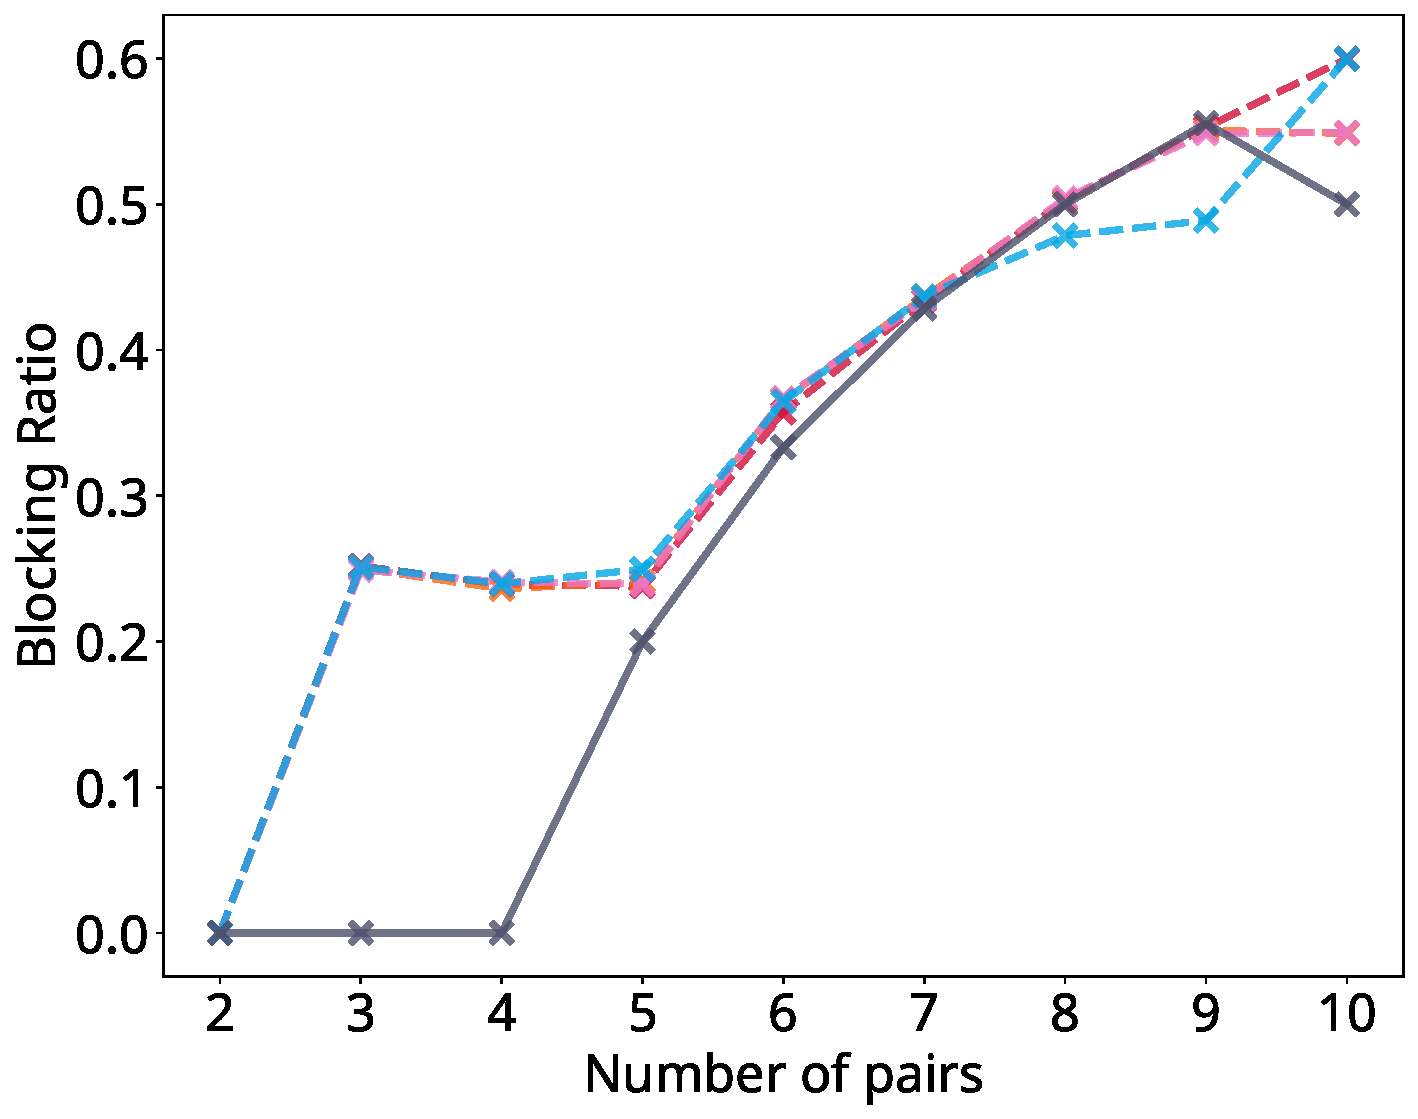
\includegraphics[width=\textwidth]{pictures/plots/n_pairs/x-2-1-s.pdf}
	\caption{$N=2, {\Lambda} = 1$, small topology}
	\end{subfigure}
	\begin{subfigure}{0.32\textwidth}
	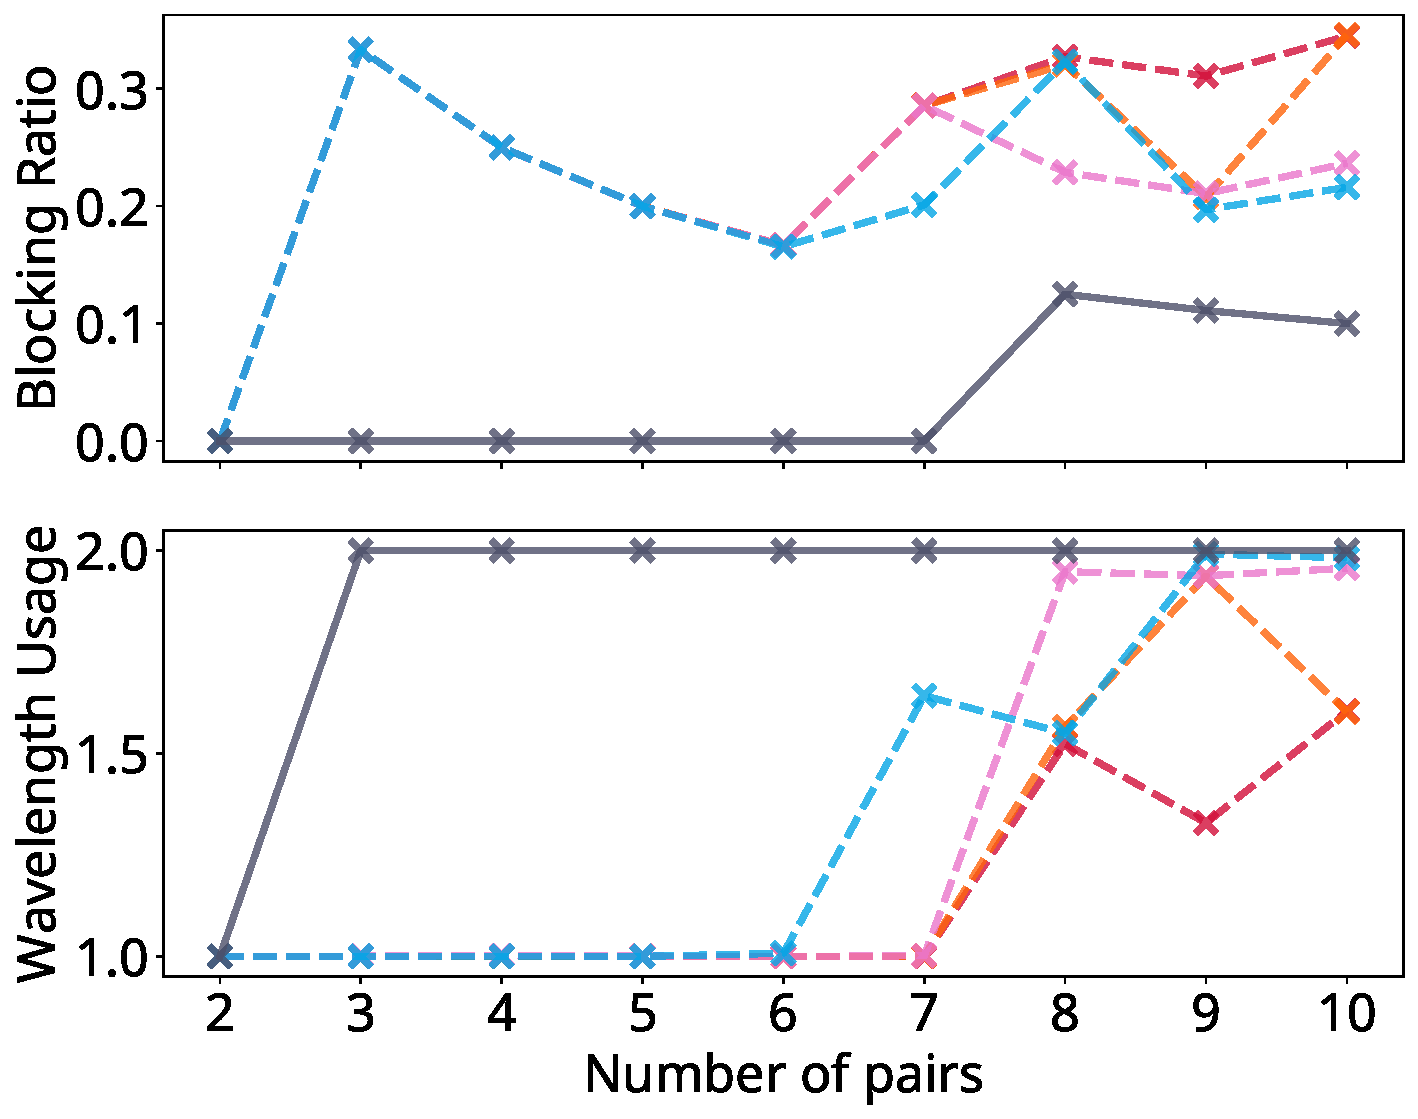
\includegraphics[width=\textwidth]{pictures/plots/n_pairs/x-1-2-m.pdf}
	\caption{$N=1, {\Lambda} = 3$, large topology}
	\label{pairb}
	\end{subfigure}
	\begin{subfigure}{0.32\textwidth}
	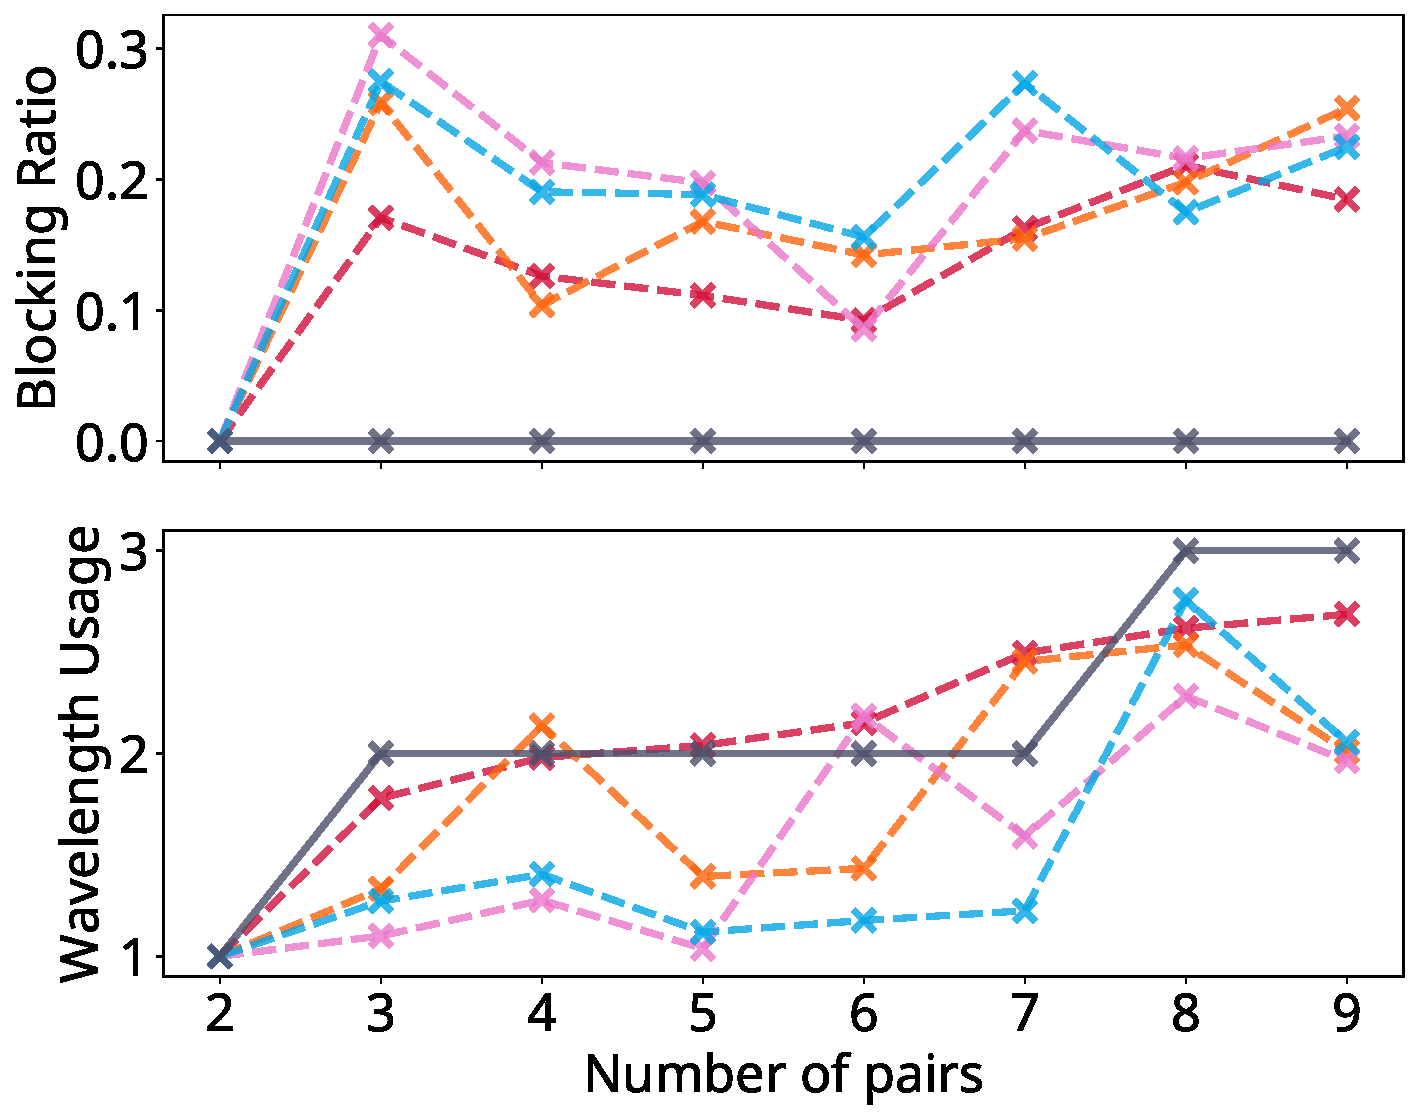
\includegraphics[width=\textwidth]{pictures/plots/n_pairs/x-1-3-m.pdf}
	\caption{$N=1, {\Lambda} = 3$, large topology}
	\label{pairc}
	\end{subfigure}
\caption{\scriptsize The blocking ratio and number of wavelength used.
\protect\reddashed is circuit depth $1$,
\protect\peachdashed is $2$,
\protect\pinkdashed is $3$,
\protect\skydashed is $4$, and
\protect\blackline is k-SPFF.
\label{fig:pairs}
}
\end{figure}
